\chapter*{Sistemi di Riferimento}
\addcontentsline{toc}{chapter}{Sistemi di Riferimento}
\section*{Introduzione}
\addcontentsline{toc}{section}{Introduzione}

Scendendo più nel dettaglio, qui è dove riportiamo le convenzioni che abbiamo adottato sui vari sistemi di riferimento utilizzati durante l’esecuzione degli esperimenti. 

Come mostrato in figura ~\ref{fig:SistemidiRiferimento} abbiamo deciso di adottare le seguenti terne: 
\begin{itemize} 
    \item \verb Sistema  \verb Fisso  \textbf{Vicon}  \verb (V)  : ha l’origine coincidente col centro della flight room; Gli assi \textbf{[ $X_{v}$ , $Y_{v}$ , $Z_{v}$]} sono fissi e rappresentano dunque il frame inerziale. 
    \item \verb Sistema  \verb Fisso   \textbf{Start}  ($S_{\#}$)  : ha l’origine coincidente con il \verb CDM  del \verb Drone  al momento dell’accensione. Ha dunque quota \textbf{“z”} nulla e, oltre ad essere complanare al sistema \textbf{“V”}, ha anche la sua stessa orientazione. Questo è il frame \verb navigation . 
    \item \verb Sistema  \verb Body  \textbf{Start} ($S_{i}$)  : Ha l’origine coincidente con il CDM del Drone in ogni istante \textbf{$t_{i}$}. Gli assi sono in ogni momento orientati in modo che l’asse \verb X  parta dall’origine e vada verso prua, l’asse \verb Y  parta dall’origine e vada verso sinistra (rispetto all’asse \verb X)  , l’asse \verb Z  che va dall’origine verso l’alto (\verb terna  \verb destrorsa). Rispetto ai due sistemi precedenti, la sua orientazione varia soltanto in termini di Yaw in quanto gli angoli di Pitch e Roll sono sempre supposti pari a zero. In questo modo evitiamo sia di considerare il relativo rumore nella misura di tali angoli da parte del sistema di visione, sia riusciamo a operare con sistemi di riferimento complanari (o “paralleli” nel caso prendano quota \verb z  > 0 ).
\end{itemize}
\\
Per quanto riguarda le misure fornite dal Vicon, queste sono tutte espresse in terna fissa \verb V . La parametrizzazione scelta per rappresentare posizione e orientazione del Drone all’interno del sistema \verb V   è la parametrizzazione \textbf{RPY } detta anche \textbf { XYZ }.
\\
Dato che il Drone, una volta acceso, crea il suo sistema \verb Body  in modo che abbia origine e orientazione coincidenti con quelle che assume all’istante di accensione, e dato che considera (per come abbiamo dovuto implementare il progetto) ogni riferimento in ingresso come espresso in un sistema la cui origine coincide con quela del \verb navigation  ma il cui frame è costantemente ruotato sull'asse \verb z  di un angolo pari al suo attuale angolo di \verb yaw  , abbiamo dovuto operare la conversione tra i due sistemi \textbf{V} ed {$S_{i}$} (rappresenta il sistema body del drone al generico istante \textbf{i}).
\\


\section*{Calcolo della matrice di Rotazione da \{Vicon\} a \{Body\}}
\addcontentsline{toc}{section}{Calcolo della matrice di Rotazione da \{Vicon\} a \{Body\}}
\\
Il Tracker fornisce roll ($\alpha$) pitch ($\beta$) yaw ($\gamma$) del drone rispetto al sistema di riferimento fisso Vicon \{V\}. Costruiamo dunque le varie matrici di rotazione che compongono la parametrizzazione di \textbf{Eulero XYZ} :

%
$$ R_{x} = 
\begin{bmatrix}
   1 & 0 & 0 \\
   0 & \cos(\alpha) & -\sin(\alpha)  \\
   0 & \sin(\alpha) & \cos(\alpha)
\end{bmatrix}
R_{y} = \begin{bmatrix}
   \cos(\beta) & 0 & \sin(\beta) \\
   0  & 1 & 0  \\
   -\sin(\beta) & 0 & \cos(\beta)
\end{bmatrix}
R_{z} = \begin{bmatrix}
  \cos(\gamma) & -\sin(\gamma) & 0 \\
  \sin(\gamma) & \cos(\gamma) & 0 \\
  0 & 0 & 1
\end{bmatrix}
$$
\\
In generale, introducendo soltanto per questo paragrafo una notazione più semplice, abbiamo un sistema \{V\} che costituisce il sistema inerziale e un sistema \{D\} che costituisce il sistema body del drone.
Questo sistema \{D\} solidale al drone ha il suo asse \verb X  rivolto da poppa a prua, asse \verb Y  in modo da avere una terna destrorsa con asse \verb Z  rivolto verso l'alto. 
Per riportare un vettore $P^v$ espresso in  \{V\} in un vettore $P^d$ espresso in \{D\} dobbiamo scrivere la: $P^d = R_{dv}\cdot P^v$ 
in cui la $R_{dv}$ esprime come passare "graficamente" da \{D\} a \{V\} (Per portare in realt\`a \{V\} in \{D\}). 
\\
Attraverso il prodotto delle 3 matrici otteniamo la matrice  $R_{xyz}$  che mappa un vettore in terna \{D\} in un vettore in terna \{V\}:
$$
R_{xyz} = R_{x} \cdot R_{y} \cdot R_{z} = R_{d}^v
$$
$$
R_{d}^v = \begin{bmatrix}
    \cos(\gamma)\cos(\beta) & -\cos(\beta)\sin(\gamma) & \sin(\beta) \\
    \cos(\alpha)\sin(\gamma) + \cos(\gamma)\sin(\alpha)\sin(\beta) & \cos(\alpha)\cos(\gamma) - \sin(\alpha)\sin(\beta)\sin(\gamma) & -\cos(\beta)\sin(\alpha) \\
    \sin(\alpha)\sin(\gamma) - \cos(\alpha)\cos(\gamma)\sin(\beta) & \cos(\gamma)\sin(\alpha) + \cos(\alpha)\sin(\beta)\sin(\gamma) & \cos(\alpha)\cos(\beta)
\end{bmatrix}
$$
\\
La $(R_{d}^v)$ per noi esprime come passare "graficamente" da V a D dunque ci\`o che ci serve 
\`e la sua trasposta:
$$
R_{v}^{d} = R_{zyx} = (R_{d}^v)^T
$$
$$
R_{v}^{d}=\begin{bmatrix}
    \cos(\gamma)\cos(\beta) & \cos(\alpha)\sin(\gamma) + \cos(\gamma)\sin(\alpha)\sin(\beta) & \sin(\alpha)\sin(\gamma) - \cos(\alpha)\cos(\gamma)\sin(\beta) \\
    -\cos(\beta)\sin(\gamma) & \cos(\alpha)\cos(\gamma) - \sin(\alpha)\sin(\beta)\sin(\gamma) & \cos(\gamma)\sin(\alpha) + \cos(\alpha)\sin(\beta)\sin(\gamma) \\
    \sin(\beta) & -\cos(\beta)\sin(\alpha) & \cos(\alpha)\cos(\beta)
\end{bmatrix}
$$
\\

\section*{Panoramica dei Sistemi di Riferimento}
\addcontentsline{toc}{section}{Panoramica dei Sistemi di Riferimento}

La figura ~\ref{fig:SistemidiRiferimento} rappresenta una panoramica “dall’alto” dunque la componente di traslazione lungo gli assi \verb z  non si vede ma sappiamo essere presente e necessaria in quanto il \verb Drone  per traslare dal suo punto di accensione deve aver prima preso quota; pertanto il sistema di riferimento {$S_{1}$}  avrà l’origine sicuramente ad una quota \verb z  > 0. I sistemi di riferimento {$S_{\#}$} , {$S_{\0}$}  e {$V$}  sono invece complanari a quota nulla. 

In fig.~\ref{fig:SistemidiRiferimento}  si mostra un esempio in cui il \verb drone  è inizialmente fermo all’istante $t_{0}$ (sistema di riferimento $S_{0}$ ), ha un angolo di \verb Yaw   pari a - $\psi_{0} $  ed è traslato rispetto al centro della stanza di $P_{vs}$ .
In realtà ad essere precisi {$S_{0}$}  esprime la reale posa del Drone rispetto all’osservatore nella stanza ma il Drone stesso crede di essere posizionato e orientato come espresso da {$S_{\#}$} (quindi con la stessa orientazione della terna {$V$}).
 
Successivamente all’istante $t_{1}$ il Drone risulta traslato rispetto al suo punto di accensione di $P_{sf}$ . Il che coincide con il dire che risulta essere traslato rispetto al centro della stanza di $P_{vf}$. 
Per tenere presente che negli istanti successivi a quello iniziale il Drone ha una quota \textbf{"z"  > 0} abbiamo indicato nel pedice delle traslazioni la lettera \textbf{f} come ultima in quanto rappresentativa della parola \textbf{fly}. 


\begin{figure}[h]
    \centering
    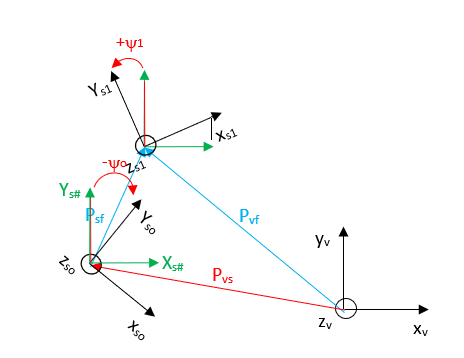
\includegraphics[width=0.8 \textwidth]{Relazione/Immagini/VICON.PNG}	
    \caption{I vari Sistemi di Riferimento introdotti}
    \label{fig:SistemidiRiferimento}
\end{figure}

Andiamo ad elencare i passaggi e le trasformazioni propri del caso rappresentato nella figura ~\ref{fig:SistemidiRiferimento}: 
\\
\begin{itemize}
    \item \textbf{Accensione del Drone in  $P_{vs}$} : il \verb Drone  crea il suo sistema di riferimento Body {$S_{0}$}  orientato come in figura.  In realtà il drone in ogni momento dell’esperimento penserà di avere angolo di \verb yaw  pari a zero in quanto noi non forniamo al filtro di Kalman le nuove misure di orientazione ma soltanto di posizione. Dunque a voler essere precisi, il Drone pensa di essere orientato esattamente come la terna {$S_{\#}$} . \\ E’ compito nostro (come vedremo di seguito) fornire riferimenti che non siano solo traslati ma anche ruotati dell’angolo di \verb Yaw  che istante per istante il drone in realtà ha rispetto a {$V$} .  
    
    \item \textbf{Creiamo dunque la matrice omogenea di rototraslazione cosi composta}:
    \\
    \\ Matrice di Rotazione da \{$S_{i}$\} a \{V\} :
    $ R_{i}^v = R_{z}(\psi_{i}) = \begin{bmatrix}
    \cos(\psi_{i}) & -\sin(\psi_{i}) & 0 \\
    \sin(\psi_{i}) & \cos(\psi_{i}) & 0 \\
    0 & 0 & 1
    \end{bmatrix}
    $
    \\
    \\
    (ricordiamo che supporremo sempre nulli gli angoli di roll e pitch)
    \\
    \\
    \\ Matrice di Rotazione da \{V\} a \{$S_{i}$\} :
    $ R_{v}^i = (R_{i}^v)^T = \begin{bmatrix}
    \cos(\psi_{i}) & \sin(\psi_{i}) & 0 \\
    -\sin(\psi_{i}) & \cos(\psi_{i}) & 0 \\
    0 & 0 & 1
    \end{bmatrix}
    $
    \\
    \\
    \\ Traslazione tra origine \{V\} e origine \{$S_{0}$\} :
    $ T_{0} = P_{vs} = \begin{bmatrix}
    x_{vs} & y_{vs} & z_{vs}
    \end{bmatrix}^T
    $
    \\
    (questa traslazione iniziale verrà continuamente convertita nella terna corrente {$S_{i}$\})
    \\
    \\
    \\ Traslazione in terna \{$S_{i}$\} :
    $ T_{si} = R_{v}^i \cdot T_{0} = \begin{bmatrix}
    \cos(\psi_{i}) & \sin(\psi_{i}) & 0 \\
    -\sin(\psi_{i}) & \cos(\psi_{i}) & 0 \\
    0 & 0 & 1
    \end{bmatrix}
    \cdot 
    \begin{bmatrix}
    x_{vs} \\ 
    y_{vs} \\
    z_{vs}
    \end{bmatrix}
    =
    \begin{bmatrix}
    x_{si} \\ 
    y_{si} \\
    z_{si}
    \end{bmatrix}
    $
    \\
    \\
    \\ Matrice Omogenea :
    $H_{si} = \begin{bmatrix}
    \cos(\psi_{i}) & \sin(\psi_{i}) & 0 & -x_{si}\\ 
    -\sin(\psi_{i}) & \cos(\psi_{i}) & 0 & -y_{si} \\
    0 & 0 & 1 & -z_{si} \\
    0 & 0 & 0 & 1
    \end{bmatrix}
    $
    \\
      \item Tralasciamo la fase di decollo in cui il \verb drone   a partire dalla sua origine iniziale prende quota lungo l’asse Z e supponiamo per semplicità di rappresentazione che non vi siano (per adesso) ulteriori rotazioni o traslazioni durante questa fase.
      \\
    \item In ogni istante il \verb Vicon  fornisce la posizione del \verb Drone  espressa nel sistema {$V$}  inizialmente pari a  $P_{vs}$  ma in generale denominata con $P_{d}^v$ che viene dunque riportata nel sistema {$S_{i}$}   prima di inviarla come misura per l’aggiornamento del filtro di Kalman. In realtà l'invio a Kalman è fatto si in ogni istante come appena detto, ma soltanto per gli istanti successivi alla fase di decollo.
    \\
    \\ Generica posizione del \verb Drone  espressa in \verb V : 
    $P_{d}^v = \begin{bmatrix}
     x_{d} & y_{d} & z_{d}   
    \end{bmatrix}^T
    $
    \\
    \\ Costruiamo il vettore omogeneo :
    $P_{dh} = \begin{bmatrix}
     x_{d} & y_{d} & z_{d} & 1 
    \end{bmatrix}^T
    $
    \\
    \\ Lo moltiplichiamo per la matrice Omogena \verb H  :
    $P_{sh} = P_{dh} \cdot H = \begin{bmatrix}
     x_{s} & y_{s} & z_{s} & 1 
    \end{bmatrix}^T
    $
    \\
    \\Lo riportiamo ad essere un vettore non omogeneo:
    $P_{d}^{si} = P_{dh} \cdot H = \begin{bmatrix}
     x_{s} & y_{s} & z_{s} 
    \end{bmatrix}^T
    $
    \\
    (Abbiamo quindi ottenuto il vettore posizione del drone non più espresso secondo la terna {$V$}  ma secondo la terna {$S_{i}$}  in quanto come detto in precedenza il drone è convinto di essere costantemente orientato come la terna {$S_{\#}$}  ed avere quindi angolo di yaw nullo. Se non avessimo proceduto alla conversione nella terna {$S_{i}$}  non sarebbe stato in grado di effettuare tale conversione in autonomia. )
    \\
    \item Supponiamo che il drone sia decollato ad esempio  ad una quota di \textbf{Z = 0.5 m} e che la Wand si trovi in posizione $P_{vf}^{v}$ (rispetto alla terna {$V$} ). Ricordiamo che l’orientazione della \verb Wand  è del tutto irrilevante ai nostri scopi e pertanto verrà sempre trascurata. A questo punto il \verb Vicon  ci fornisce $P_{vf}^{v}$ e noi la andiamo a ruotare in accordo con l'attuale orientazione della terna Body {$S_{i}$}   per poi traslarla riconducendo l'origine a quella della terna \verb navigation  . In questo modo otteniamo  come riferimento di posizione per il Drone il vettore $P_{vf}^{si}$.
    \\
    \\
    $P_{vf}^{v} = \begin{bmatrix}
       x_{vf} & y_{vf} & z_{vf}
    \end{bmatrix}^T 
    $
    , costruisco il vettore omogeneo
    $P_{vfh} = \begin{bmatrix}
       x_{vf} & y_{vf} & z_{vf} & 1
    \end{bmatrix}^T
    $
    \\
    ottengo infine : 
    $P_{vf}^{si}=H \cdot P_{vfh} = \begin{bmatrix}
       x_{sf} & y_{sf} & z_{sf} & 1
    \end{bmatrix}^T
    $
    \\
    \item A questo punto il nuovo riferimento è inviato al \verb Drone  che lo insegue. Durante il tragitto continuiamo a inviare, come prima, la sua posizione al filtro di \verb Kalman  continuando a fargli credere che il suo angolo di \verb yaw  è rimasto nullo. Possiamo farlo in quanto il riferimento che deve inseguire è già stato ruotato di conseguenza.
    \\
    \item Una volta che il \verb Drone  raggiunge la posizione desiderata, supponiamo che (a causa di eventuali disturbi durante il tragitto) abbia variato il suo angolo di \verb yaw  e che adesso sia pari a $\psi_{1}$ mostrato nella figura ~\ref{fig:SistemidiRiferimento} relativamente all’istante $t_{1}$  .  In questo caso infatti il sistema \verb Vicon  rileverà il nuovo valore dell’angolo che sarà utilizzato per ricalcolare la matrice omogenea come segue:
    \\
    \\
    \\ Matrice di Rotazione da \{$S_{1}$\} a \{V\} :
    $ R_{s1}^v = R_{z}(\psi_{1}) = \begin{bmatrix}
    \cos(\psi_{1}) & -\sin(\psi_{1}) & 0 \\
    \sin(\psi_{1}) & \cos(\psi_{1}) & 0 \\
    0 & 0 & 1
    \end{bmatrix}
    $
    \\
    \\Matrice di Rotazione da \{V\} a \{$S_{1}$\} :
    $ R_{v}^{s1} = (R_{s1}^v)^T = \begin{bmatrix}
    \cos(\psi_{1}) & \sin(\psi_{1}) & 0 \\
    -\sin(\psi_{1}) & \cos(\psi_{1}) & 0 \\
    0 & 0 & 1
    \end{bmatrix}
    $
    
    \\
    \\ Traslazione tra origine \{V\} e origine \{$S_{0}$\} :
    $ T_{0} = P_{vs} = \begin{bmatrix}
    x_{vs} & y_{vs} & z_{vs}
    \end{bmatrix}^T
    $
    \\
    \\
    \\ Traslazione ruotata in \{$S_{1}$\}  :
    $ T_{s1} = R_{v}^{s1} \cdot T_{0} = \begin{bmatrix}
    \cos(\psi_{1}) & \sin(\psi_{1}) & 0 \\
    -\sin(\psi_{1}) & \cos(\psi_{1}) & 0 \\
    0 & 0 & 1
    \end{bmatrix}
    \cdot 
    \begin{bmatrix}
    x_{vs} \\ 
    y_{vs} \\
    z_{vs}
    \end{bmatrix}
    =
    \begin{bmatrix}
    x_{s1} \\ 
    y_{s1} \\
    z_{s1}
    \end{bmatrix}
    $
    \\
    \\
    \\ Matrice Omogenea :
    $H_{s1} = \begin{bmatrix}
    \cos(\psi_{1}) & \sin(\psi_{1}) & 0 & -x_{s1}\\ 
    -\sin(\psi_{1}) & \cos(\psi_{1}) & 0 & -y_{s1} \\
    0 & 0 & 1 & -z_{s1} \\
    0 & 0 & 0 & 1
    \end{bmatrix}
    $
    \\
    \item Adesso viene ricalcolata la nuova posizione della \verb Wand  che verrà riconvertita utilizzando la nuova matrice appena calcolata per fornirla al \verb Drone  come nuovo riferimento da inseguire. Allo stesso modo continuerà ad essere inviata al filtro di Kalman la misura di posizione attuale del \verb Drone  , anch’essa fornita in sistema {$V$}  e riconvertita utilizzando la nuova matrice appena calcolata. 
    \\
    \\
    Notiamo come già ripetuto ormai più volte in precedenza che per ogni variazione all'angolo di yaw il drone continua a ricevere riferimenti di posizione da inseguire e stime della sua posizione entrambi riferiti ad un sistema posizionato sulla terna \verb navigation  ma orientata come la corrente terna \verb body  in quanto continua ad essere convinto di avere yaw nullo e pertanto noi continuiamo a inviargli informazioni in cui la "correzione" dell'orientazione è già stata calcolata.
    \\
    \item Il tutto si ripete con una frequenza di 100 Hz fin quando la \verb Wand  non viene spenta.
    \\
    \item In questo istante il sistema \verb Vicon  fornirà come posizione della Wand il valore \textbf{[0, 0, 0]}  che coincide con il valore fornito ogni qualvolta, per qualsiasi motivo, il \verb Vicon  non riesce a individuare la \verb Wand  in uno o più frame. Avendo dunque deciso di interpretare questo particolare valore di posizione come codice di errore (in quanto considerando il vincolo del pavimento e la presenza di rumore nelle misure è assolutamente improbabile se non impossibile che un oggetto si trovi in quella posizione esatta per uno o addirittura più istanti consecutivi) nel caso in cui questo venga ricevuto noi continuiamo a mantenere il drone fermo nella sua ultima posizione e, qualora il valore sia fornito per un dato numero di istanti consecutivi, decidiamo di intraprendere la fase di atterraggio per concludere quindi l’esperimento. 
    \\
\end{itemize}


